\chapter{Specification}
The specification of the program defines what it does rather than how.
This chapter presents the specification of the system taking into consideration general software engineering principles, like the models proposed by Larman (at least conceptual, use case and behaviour models) and Meyer's \ac{DbC}.
For the particular case of this thesis, the specification takes into account reengineering principles and procedures and \ac{TDD} as a tool to define what the system does as opposed to a simple testing technique.

Reengeneering a software involves reverse engineering, understanding what the system does.
The outcome of this process (FIXME: activity, task?) derives part of this specification.
For example, use cases are extracted from the current system.

There are 3 key issues in understanding the current system: abstraction level, completeness and direction.
This specification uses a system-level abstraction, only takes into account interaction with external actors, and is one-way (from current system to the specification of the new system).
Other levels of abstraction do not apply here to keep this specification technology-agnostic.


\section{Interaction, interoperability and context}

\subsection{Context}
\begin{figure}[htb]
    \label{fig:context-original}
    \centering
    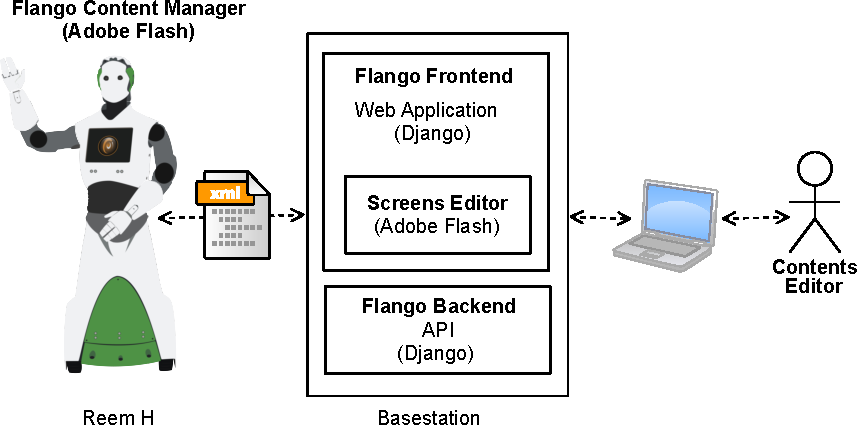
\includegraphics[width=\textwidth]{figures/context-original}
    \caption{Current context}
\end{figure}

\begin{figure}[htb]
    \label{fig:context-new}
    \centering
    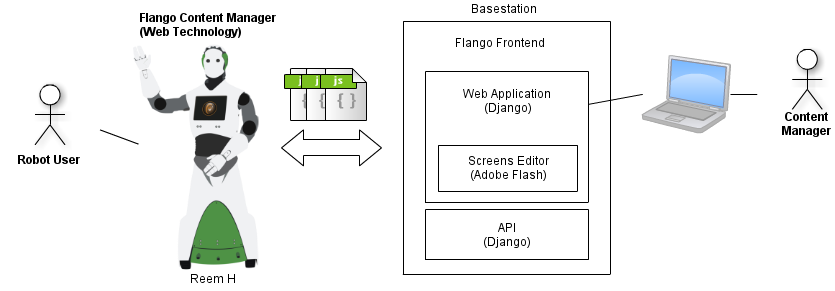
\includegraphics[width=\textwidth]{figures/context-new}
    \caption{New context}
\end{figure}

Key aspects when understanding the current program include the interaction, interoperability and the context.
ReemH-3 has about 600MB of specialised code and uses up to 13GB to store the operating system, libraries and other tools.
The program that manages the state machine is \textbf{robotBehaviour}, a \texttt{Qt} program that glues all software parts and serves as an interface to the hardware.
A dialog in this program contains a QtWebKit widget, the embedded web browser that loads the contents shown in the touchscreen.
Contents are fetched from Basestation, a server that hosts \textbf{Flango Frontend}, a web application (Django + Flash) that lets users edit screens, add media contents and synchronise them with robots (\fref{fig:context-original}).
The Frontend has an \ac{API} to serve the contents applications to the robots.
The project of this thesis is reengineering the \textbf{Flango Content Manager}, in the robot (\fref{fig:context-new}).

\subsection{Interaction}
\begin{figure}[htb]
    \label{fig:interaction-original}
    \centering
    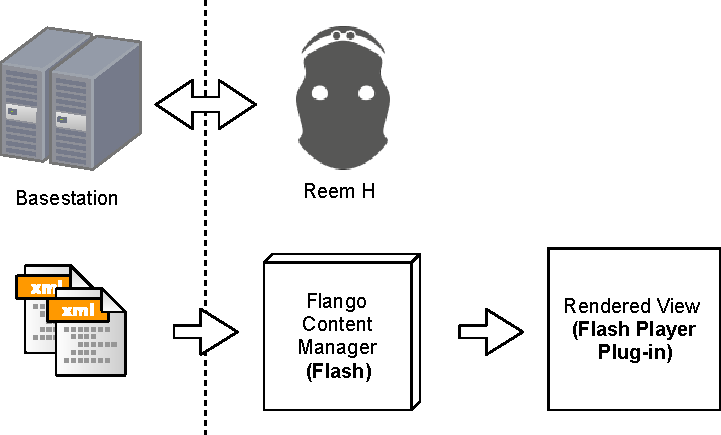
\includegraphics[width=0.7\textwidth]{figures/interaction-original}
    \caption{current interaction}
\end{figure}

\begin{figure}[htb]
    \label{fig:interaction-new}
    \centering
    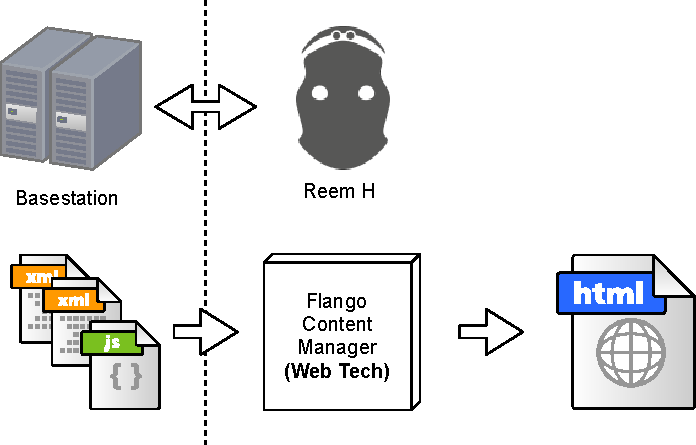
\includegraphics[width=0.7\textwidth]{figures/interaction-new}
    \caption{New interaction}
\end{figure}

The content manager's input is \ac{XML} files and the output is an \ac{HTML} single page application (\fref{fig:interaction}).

\begin{enumerate}
    \item The robot boots
    \item robotBehaviour fetches settings (\ac{XML}) from Basestation: generic settings, contents application-specific settings and the structure.
    \item The Content Manager uses the settings to decide which application to load, the language, the theme, etc. and requests the screens (the \ac{XML} files) to Basestation
    \item Basestation serves all the screens
    \item The Content Manager renders the screens. If during this process encounters an "entity", it fetches the data from Basestation.
\end{enumerate}


\subsection{Interoperability}
\begin{figure}[htb]
    \label{fig:interoperability-original}
    \centering
    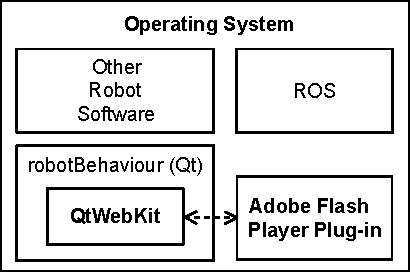
\includegraphics[width=0.7\textwidth]{figures/interoperability-original}
    \caption{Current interoperability (in robot)}
\end{figure}

\begin{figure}[htb]
    \label{fig:interoperability-new}
    \centering
    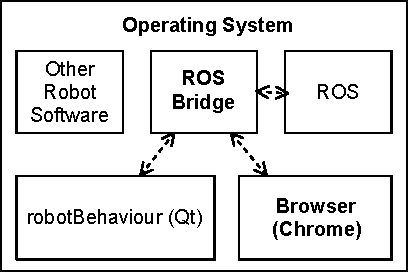
\includegraphics[width=0.7\textwidth]{figures/interoperability-new}
    \caption{New interoperability (in robot)}
\end{figure}

Flango Content Manager interoperates with two systems: robotBehaviour and Basestation.

\paragraph{robotBehaviour} Flango can interact with the hardware of the robot through robotBehaviour, e.g. using text-to-speech capabilities, triggering a batch action (autopresentation, guide user to a certain place...).
Likewise, robotBehaviour uses an API in Flango, e.g. to restart a session or to input information gathered with the robot's hardware.
There is an interface defined for this to allow independent development in both ends.
Notice that figures \fref{fig:interoperability-original} and \fref{fig:interoperability-new} do not show Basestation. See \fref{fig:context-original} and \fref{fig:context-new}.
The current system to exchange messages between the Flash container and robotBehaviour is based on JavaScript callbacks.
To send a message to robotBehaviour:
\begin{enumerate}
    \item Flash opens a new tab with a specific url: \texttt{flashCallback.html?\textless paramList\textgreater}
    \item robotBehaviour intercepts the call, prevents QtWebKit from opening a new tab and executes an action specified with the parameters
\end{enumerate}

To send a message from robotBehaviour:
\begin{enumerate}
    \item Calls a \ac{JS} function in the Flash container (\texttt{/static/frontend/index.html})
    \item The container forwards this call to the Flash container
    \item The application facade of Flango Content Manager takes required action
\end{enumerate}

The requirements state that the new software has to be implemented using web technology. 
Despite the fact that this specification should be technology agnostic, to integrate the new software better in the system, the use of ROS Web Tools is suggested to exchange messages.
In any case, it is clear that there has to be an interface between robotBehaviour and the browser, as they run in separate processes (as opposed to sharing at least one parent process in the current implementation).

\paragraph{BaseStation (Flango Backend API} The Content Manager has to fetch data from Basestation in order to load the correct contents.
Flango Backend (TODO EPIC FIXME. fix the diagrams and everything. BS has backend and frontend) has an API for this:

\begin{table}[ht]
    \centering
    \caption{Flango Backend API}
    \label{tab:milestones}
    \begin{tabularx}{\linewidth}{| l | X |}
    \hline
    Root URL & Matching URLs \\
    \hline
    \multirow{2}{*}{$flango-api-0.1/robots$}
        & get\_robots \\ 
        & add\_robot \\
    \hline 
    
    \multirow{2}{*}{$flango-api-0.1/bl$} 
        & entity/(\textless entity\_name\textgreater).xml \\ 
        & add\_robot \\
    \hline
    
    \multirow{6}{*}{$flango-api-0.1/pal$} 
        & home \\
        & add \\
        & execute \\
        & status \\   
        & submit \\
        & history/(\textless page\textgreater) \\
    \hline
    
    \multirow{10}{2.5cm}{\texttt{flango-api-0.1/gui}  \texttt{flango-api-0.1/app}}
        & \textless app\_id\textgreater /config.\textless format\textgreater xml$|$json \\
        & \textless app\_id\textgreater /structure.\textless format\textgreater xml$|$json \\
        & \textless app\_id\textgreater /screen/( \textless screen\_id\textgreater.xml \\
        & \textless app\_id\textgreater /node/\textless node\_id\textgreater \\
        & application \\
        & node \\
        & screen \\
        & allScreens \\
        & getApps \\
        & upload\_app \\
    \hline
    \end{tabularx}
\end{table}

Both current and new implementation use this.
However, the new implementation uses \ac{JSON} because it is more \ac{JS}-friendly: it has less overhead and it is easier to deserialise.

\section{conceptual model}

classes of objects: setting, ui component (basic, theme), "entity". 
constraints?

\section{use case model}
system actors:
robotbehaviour, system
Users: no users (well, a "virtual" user does exist). it's a meta-app that reads apps in xml and renders them in html. define input and output.


system use cases:
configure app (generic settings, app-specific settings, structure with nodes and screens)
render UI (define XML syntax here. XML (vocabulary, grammar, motivations). one sub-usecase per UI component?)
render entity (use render UI)
navigate to URI
interoperate with robotBehaviour 

\section{behaviour model}
seq diagrams of system operations

This thesis combines design by contract and tdd. basically, tests define the behaviour for specific cases and dbc defines the general behaviour. thus, there are no tests for edge cases or negative behaviours because conracts, and more specirfically preconditions, protect the component.
Advantages:
with tdd:
build only what is required now. keep it simple.
have a suite of automated tests for refactoring safely, continuous integration and regression testing.
drive design decisions from tests (from specs).
using formal specs (dbc):
higher code quality
less checks (preconditions)
design decisions derived from preconditions

Larman: system sequence diagram + Meyer: contracts of system operations
%http://citeseerx.ist.psu.edu/viewdoc/download?doi=10.1.1.68.313&rep=rep1&type=pdf
"System Sequence Diagrams:
–
Identify system events and system operations
–
Identify system events and system operations
– Document sequence of interactions
• Contracts:
– Define the pre- and post-conditions for system
operations "


TDD specs:
clarify this is here because we write tests before writing code. tests are implemented with a certain framework and oriented to a certain technology but this chapter focuses on what the tests say and why we do it this way.
outline tests


Design by Contract and Test Driven Development are not at all mutually exclusive.
TDD is not about testing!! is about executable specs
"The first idea is about test-driven development not being a testing technique;
automatic tests only become ”tests” after having implemented all the functionality
being test-
driven
. Before that there is nothing to actually
test
and those artifacts
rather serve as executable
specifications
but not tests"

up to date documentation: a common problem is that docs are hardly ever updated


---
Extreme Programming advocates test driven development where tests are used
to specify the behavior of a program before the program code is actually written.
Together with using the simplest design possible and intention revealing program
code, tests are additionally used as a documentation of the program. However,
tests are not sufficient to completely define the behavior of a program because
they are only able to test properties of a program by example and do not allow to
state general properties. The latter can be achieved using formal specifications,
e.g. using Meyer’s design by contract % http://citeseerx.ist.psu.edu/viewdoc/download?doi=10.1.1.68.313&rep=rep1&type=pdf